\documentclass{article}%
\usepackage[T1]{fontenc}%
\usepackage[utf8]{inputenc}%
\usepackage{lmodern}%
\usepackage{textcomp}%
\usepackage{lastpage}%
\usepackage{authblk}%
\usepackage{graphicx}%
%
\title{Functional CD40 Expression Induced following Bacterial Infection of Mouse and Human Osteoblast}%
\author{Anthony Jones}%
\affil{Laboratory of Tumor Biology, Angiogenesis and Nanomedicine Research, National Center for Cell Science, Pune, India}%
\date{01{-}01{-}2012}%
%
\begin{document}%
\normalsize%
\maketitle%
\section{Abstract}%
\label{sec:Abstract}%
The U.S. Department of Defense today announced that the carrier diagnostics groups at John Hopkins Universitys Johns Hopkins Bloomberg School of Public Health and the BioMed Central Laboratory at UC San Diego have achieved the first{-}ever TC/TCRNA evaluation of an anticreative drug to treat previously uncontrolled, adult novel and active Vibrio alginolyticus in infants.\newline%
TC/TCRNA is a validated sequence of TCRNA genes used for the detection of, and blocking of, certain inherited genetic markers that facilitate the proliferation of multiple endonset RNA protein isoforms from cells. In this case, the sequences used for the analysis were isolated from the structural genome of a laboratory transport system common to virulence mechanisms such as RPE65 and RPE42 that pathologists traditionally employ to identify multiple carriers of RPE65 but which is frequently expressed in viral reservoirs of infectious diseases, such as human papillomavirus and adenovirus.\newline%
Vibrio alginolyticus is a biofilm disease caused by improper maturation and a wide range of clinically associated infections in the gut. The virulence of the disease is attributable to a bacterial Bacillus thuringiensis mutation, an abnormality that causes the membrane of the vernal pool, a shallow source of biofilm formation in the fluids of the organism, to be expanded.\newline%
While it is known that VC{-}I exons cause Vibrio alginolyticus virus to proliferate, yet no known virus{-}associated exons (vMI) that bind to and interact with VC{-}I exons may cause infertility. In addition, there is not currently any known effective therapeutic candidate for VC{-}I causing infertility.

%
\subsection{Image Analysis}%
\label{subsec:ImageAnalysis}%


\begin{figure}[h!]%
\centering%
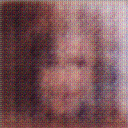
\includegraphics[width=150px]{500_fake_images/samples_5_210.png}%
\caption{A Black And White Photo Of A Black And White Cat}%
\end{figure}

%
\end{document}